\documentclass{cernyrep}
%\usepackage{texnames}
\usepackage[T1]{fontenc}
\sloppy
\usepackage[bookmarks, colorlinks=true, linktoc=page, pdftex, linkcolor=black, citecolor=black, urlcolor=blue]{hyperref}
%\pagestyle{empty}
\pagestyle{plain}
\usepackage{fancyhdr}
\usepackage{ctex}
%\fancyhfoffset: System command execution is disabled (see Preferences)
\fancyhfoffset{4 mm}
\fancypagestyle{ARTTITLE}{% 
\fancyhf{} % clear all header and footer fields
\lhead{\hfill CERN Accelerator School Proceedings ---
{\it RF for Accelerators} ---  Berlin, Germany,  2023\hfill}
\lfoot{\hspace{3mm} Available online at \url{https://cas.web.cern.ch/previous-schools}}
\rfoot{\thepage\hspace*{3mm}}
\renewcommand{\headrulewidth}{0.1pt} 
\renewcommand{\footrulewidth}{0.1pt}
}

% define \der{#1}{#2} as a shortcut for the derivative
\newcommand{\der}[2]{\frac{\mathrm{d}#1}{\mathrm{d}#2}}
% define \pder{#1}{#2} as a shortcut for the partial derivative
\newcommand{\pder}[2]{\frac{\partial#1}{\partial#2}}
% \rd for the roman d in math mode for integrals and derivative
\newcommand{\rd}[0]{\mathrm{d}}

\renewcommand{\textfraction}{0.1}
\renewcommand{\topfraction}{0.9}
\renewcommand{\bottomfraction}{0.9}

\usepackage{varwidth}
\usepackage{xcolor}
\frenchspacing
%%%%%%%%%%%%%%%%%%%%%%%%%%%%%%%%%%%%%%%%%%%%%%%%%%%%%%%%%%%%%%%%%%%%%%%

\begin{document}

\title{匹配与功率耦合}
\author{Graeme Burt}
\institute{英国兰卡斯特大学科克克罗夫特研究所}

\begin{abstract}
在任何射频系统中，一个关键因素是将射频功率从放大器耦合到加速腔中的机制。若传输线与其负载之间存在阻抗失配，任何传输线都会产生反射。由于加速腔具有很高的品质因数，腔体并联阻抗与传输线之间常常存在较大的失配。本讲将讨论如何克服这种失配，并在驻波腔和行波腔中实现高效耦合且在稳态下无反射。
\end{abstract}
\keywords{阻抗匹配；射频耦合。}
\maketitle
\thispagestyle{ARTTITLE}

\section{引言}
射频通过波导或其他任何传输线耦合进射频腔并从中耦出。耦合器可以采用矩形波导或同轴结构。腔体与耦合器之间的接口可以通过电场、磁场或二者同时进行耦合。在接口处，入射波可以传入腔体，也可以反射回传输线。使进入腔体的传输最大化并使反射最小化的过程称为匹配。
\section{射频耦合器}\index{模式匹配}
在两个射频区域的接口处，为满足麦克斯韦方程，场必须在接口处连续，也就是说接口两侧的电场和磁场必须相同。除此之外，任何金属壁面的边界条件也必须保持，$E_{||}=H_t=0$。如果两个射频区域的横截面不同，就不可能将一侧的单一模式与另一侧的单一模式完全匹配，因此会发生多模耦合。对于波导耦合器，波导模式中的场（通常为$\textrm{TE}_{10}$模式）应与腔内场相匹配，并使接口两侧的电场和/或磁场方向一致。电场之间的耦合可通过将接口处的腔体场$\vec{E_{cav}}$与耦合器内模态展开式匹配得到
\begin{equation}
    \vec{E_{cav}}= \sum_{n=1}{a_n \vec{E_{n,coup}}},
\end{equation}
其中，$\vec{E_{n,coup}}$是该接口处第$n$个波导模的电场，$a_n$是该波导模的幅度。类似地，腔体接口处的磁场$\vec{B_{cav}}$可展开为
\begin{equation}
    \vec{B_{cav}}= \sum_{n=1}{a_n \vec{B_{n,coup}}},
\end{equation}
其中，$\vec{B_{n, coup}}$是接口处第$n$个波导模的磁场，$a_n$是该波导模的幅度。可对每个波导模求解该方程，从而得到各模态的耦合。
然而，同时匹配电场和磁场不能只靠一个系数实现。在任何不连续接口处，朝向该接口传播的波都会被散射成前向波和后向波。根据不连续类型，前向波和后向波的电场会相加或相减，而磁场则相反。这意味着通过引入后向波，我们可以同时匹配接口处的两组场。此时电场为：
\begin{equation}
    \vec{E_{cav}}= \sum_{n=1}{a_n \vec{E_{n,coup}}} + \sum_{n=1}{b_n \vec{E_{n,coup}}},,
\end{equation}
其中，$a_n$是前向（入射）波导模的幅度，$b_n$是后向（反射）波导模的幅度。若考虑一个连接腔体与波导的孔径，可以用波导中的正弦傅里叶级数来重现腔体在孔径处呈现的场。除非腔体场在孔径上正好是半个周期，否则波导中会存在多个空间谐波。由于波导中的场被离散为不同模态，横向宽度上有$m$个半波变化、纵向高度上有$n$个半波变化，因此傅里叶级数中的每个谐波都对应一个不同的波导模。由于存在前向波和反向波，这本来不是单值问题，但同时匹配电场和磁场的要求会将其约束为一个由有限个模幅组成的唯一解。由于大多数波导功率耦合器在其工作频率下只设计有一个高于截止的模，其余模都会截止。这些截止模局限在接口附近，并向波导内部指数衰减，但它们仍然很重要，因为它们会吸收功率并在耦合孔附近局部提高场强。

对于同轴耦合器，我们可以在耦合器末端、即腔体与耦合器相接之处优化其几何结构，以确保腔体达到临界耦合。若内导体末端不连接外导体（称为探针式终端），如图~\ref{fig_Probetypes}所示，则腔体电场可在内外导体之间产生随时间变化的电荷差，因此等效为一个与内外导体间电容并联的电流源。电流$I$为
\begin{equation}
    I=- \frac{\mathrm{d}Q}{\mathrm{d}t} = -\epsilon_0 \frac{\mathrm{d} \int_{tip}{\vec{E}.\mathrm{d}\vec{S}}}{\mathrm{d}t},
\end{equation}
其中，$E$是内导体尖端处的电场，$S$是内导体尖端的表面积。
如果通过一个环将内导体与外导体连接，那么磁场可通过电磁感应在该环上产生电压。这对应的等效电路为一个串联电感的电压源。电压为
\begin{equation}
    V=- \frac{\mathrm{d} \Phi}{\mathrm{d}t} = - \frac{\mathrm{d} \int_{loop}{\vec{B}.\mathrm{d}\vec{S}}}{\mathrm{d}t},
\end{equation}
其中，$\Phi$是穿过回路的磁通量。磁环在装配上较为困难，因为需要将内外导体连接起来。也可以在同轴线内导体末端采用一个感应式“钩形”结构，并在其与外导体之间留有一个小电容间隙，如图~\ref{fig_Probetypes}所示。这样的终端既可被电场激励，也可被磁场激励，但二者的等效电路略有不同。对于钩形结构，电感和电容彼此串联；而对于磁场耦合，该串联LC电路还与电压源串联；对于电场耦合，该串联LC电路则与电流源并联。由于电容$C_{gap}$与电感$L_{loop}$串联，它们形成一个谐振电路，对电场表现为带阻滤波器，对磁场表现为带通滤波器，其谐振频率为
\begin{equation}
    \omega_f=\frac{1}{L_{loop} C_{gap}}.
\end{equation}
各类耦合方式的等效电路如图~\ref{fig_HOMcouplingcircuit}所示。具体选择哪一种，取决于耦合器位置、该位置的腔体场分布以及耦合器尖端的射频热负荷。

\begin{figure}
\centering
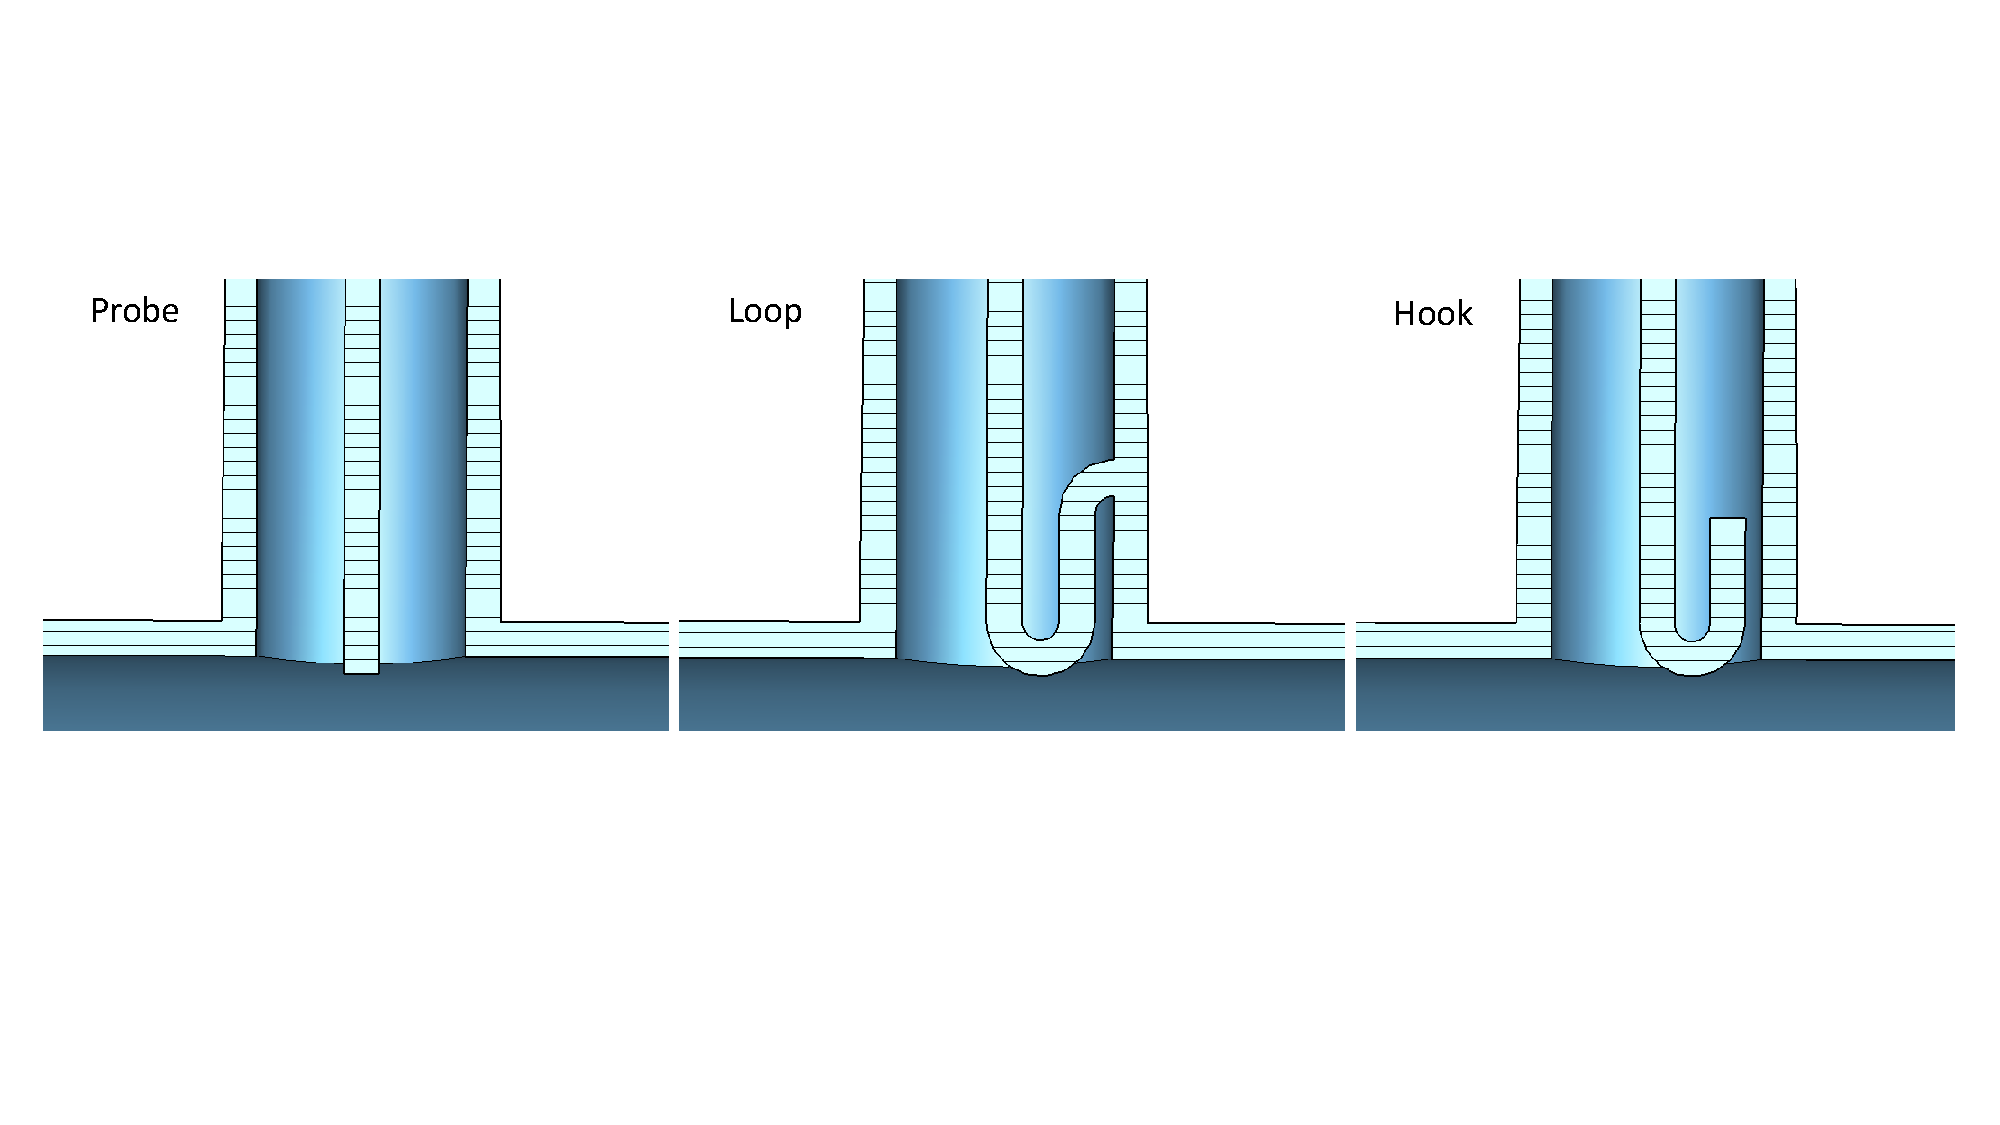
\includegraphics[width=120mm]{figures/Probetypes.pdf}
\caption{\label{fig_Probetypes} 同轴耦合器的三种终端形式：探针、环形和钩形。}
\end{figure}

\begin{figure}
\centering
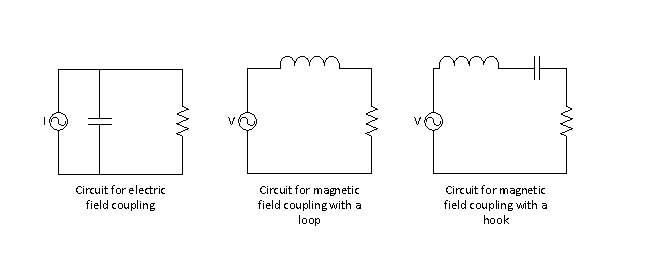
\includegraphics[width=120mm]{figures/HOMcouplingcircuit2.pdf}
\caption{\label{fig_HOMcouplingcircuit} 电耦合与磁耦合的等效电路。}
\end{figure}

\subsection{Coupling Power into an RF Structure}
为了将射频（RF）功率源连接到腔体，必须构造一个能向腔体辐射功率的天线，以避免功率被沿波导反射回去。通常这就是通过波导或同轴线，经束管或腔壁上的小孔与腔体连接的输入或功率耦合器（input 或 power coupler），将在后文讨论。腔体与耦合器之间存在不连续性并且阻抗不匹配，导致反射。同时进入腔体的一部分功率又会耦合回耦合器，反射波与腔体发出的功率相叠加并相互干涉。随着腔体内存储能量增加，泄回耦合器的功率也增加，向后的行波随时间变化直到腔体达到稳态。

耦合强度可用外部品质因数$ Q_e $表示，它把腔体内的存储能量与在无外加驱动时会流入耦合器的功率$ P_e $联系起来：\index{Q factor}
\begin{equation}
Q_e= \frac{\omega U}{P_e}.
\end{equation}
当输入功率关闭时，将流入耦合器的外部功率$ P_e $与腔体的欧姆损耗$ P_c $相加得到总损耗$ P_t $（即$ P_t = P_e + P_c $），由此可定义包含所有损耗的加载品质因数$ Q_L $，对于单耦合器腔体有
\begin{equation}
\frac{1}{Q_L} = \frac{1}{Q_0} +  \frac{1}{Q_e} .
\end{equation}
同时定义耦合因子$ \beta $为耦合器损耗与腔壁欧姆损耗之比：
\begin{equation}
\beta = \frac {P_e}{P_c} = \frac{Q_0}{Q_e}.
\end{equation}

腔体在有限带宽内可以耦合功率。由等效电路作为频率 $ \omega $ 的函数可求得腔体阻抗：
\begin{equation}
    Z=\frac{R_{s,circuit}}{1+i Q_L \left( \frac{\omega}{\omega_0}-\frac{\omega_0}{\omega}\right)}.
\end{equation}
由此在 Z 上的半高全宽带宽为 $2 Q_L/\omega$。

在该带宽之外的频率，所有功率将被反射。对一个方波脉冲，其上升和下降沿包含宽频带分量，其中部分落在腔带外而被反射。对于缓慢上升沿或较大的腔带宽，反射量较少。为建模此过程，可用等效电路来描述。耦合器阻抗通常为几十欧姆以便高功率传输，而为达到高场梯度腔体阻抗可达数兆欧，因此二者在接口处存在很大的阻抗失配，产生接近反相的强反射。接口反射与由腔体向耦合器泄出的功率相叠加，驱动腔体在谐振时沿耦合器向外的总功率$ P_r $为：
\begin{equation}
\label{eqn_ReflectU}
P_r= \Bigg(\sqrt{P_f}-\sqrt{ \frac{\omega U}{Q_e}} \Bigg)^2,
\end{equation}
其中$ P_f $为来自射频源的前向功率。将返回波定义为反射功率$ P_r $，空腔时的接口反射记为$ P_i $，腔体泄出的功率记为$ P_e $。

在无束情况下，腔体内存储能量随时间的变化由流入与流出功率之和给出：
\begin{equation}
\frac {\mathrm{d}U}{\mathrm{d}t}= P_f-\Bigg(\sqrt{P_f}-\sqrt{ \frac{\omega U}{Q_e}} \Bigg)^2-\frac{\omega U}{Q_0}.
\end{equation}
展开可得：
\begin{equation}
\frac {\mathrm{d}U}{\mathrm{d}t}= \sqrt{ \frac{4 P_f \omega U}{Q_e}}-\omega U \Big( \frac{1}{Q_0} +  \frac{1}{Q_e} \Big)
\end{equation}
代入加载 Q 的定义得：
\begin{equation}
\frac {\mathrm{d}U}{\mathrm{d}t}= \sqrt{ \frac{4 P_f \omega U}{Q_e}}- \frac{\omega U}{Q_L}.
\end{equation}

令稳态时 $\mathrm{d}U/\mathrm{d}t=0$，解关于 $\sqrt{U}$ 的二次方程可得稳态存储能量 $U_0$：
\begin{equation}
\label{eqn_U0}
U_0 =  \frac{4 P_f Q_L^2}{Q_e \omega}= \frac{4 P_f \beta}{(1+\beta)^2} \frac{Q_0}{\omega},
\end{equation}
并可变形求得为达到给定腔电压所需的前向功率：
\begin{equation}
\label{eqn_Pf}
P_f =  \frac{V_c^2 (1+\beta)^2}{8 R \beta}.
\end{equation}

假设初始能量为零，求解时间依赖解得：
\begin{equation}
\label{eqn_Uvst}
U = U_0  \bigg( 1 - e^{-\omega t/2 Q_L} \bigg)^2.
\end{equation}
腔体填充时间常数 $\tau$ 为：
\begin{equation}
\tau=\frac{\omega}{Q_L},
\end{equation}
因此填充速率与加载 Q 成反比。将 Eq.~(\ref{eqn_U0}) 代入 Eq.~(\ref{eqn_ReflectU}) 可得稳态反射功率：\index{reflected power}
\begin{equation}
P_r= P_f \Bigg( 1- \frac{2 Q_L}{Q_e} \Bigg)^2
\end{equation}
或写成耦合因子形式：
\begin{equation}
P_r= P_f \Bigg( 1- \frac{2 \beta}{1+ \beta} \Bigg)^2.
\end{equation}

当 $\beta=1$ 时，反射功率为零，称为临界耦合（critically-coupled）。此时接口反射与腔体向外发射的功率幅值相等且相差 180$^\circ$，相互抵消。$\beta>1$ 为过耦合，$\beta<1$ 为欠耦合。由稳态反射测得耦合因子的公式为：
\begin{equation}
\beta= \frac{1 \pm \sqrt{P_r/P_f}}{1 \mp \sqrt{P_r/P_f}},
\end{equation}
上号适用于 $\beta>1$，下号适用于 $\beta<1$。常把 $\sqrt{P_r/P_f}$ 记为输入端口反射系数 $S_{11}$。将 Eq.~(\ref{eqn_Uvst}) 代入 Eq.~(\ref{eqn_ReflectU}) 可得到时变反射功率表达式：
\begin{equation}
P_r= P_f \left[ 1- \frac{2 \beta}{1+ \beta} \bigg( 1 - e^{-\omega t/2 Q_L} \bigg) \right]^2.
\end{equation}
此处第一项为接口反射，第二项为腔体发射项。对于临界或欠耦合情况，起始时反射接近 100\%，随腔内能量增加被逐渐抵消；过耦合时则会出现先降到零再上升的现象，且反射相位在穿越零点时改变 180$^\circ$，如图~\ref{fig:superposition} 所示。

当射频突然关闭（$P_f=0$）时，发射项不再被前向功率抵消，关断瞬间的峰值反射功率为：
\begin{equation}
P_r= \frac{\omega U}{Q_e} = P_f \Bigg(  \frac{2 \beta}{1+ \beta} \Bigg)^2,
\end{equation}
过耦合时该峰值可达前向功率的 4 倍，临界耦合时等于前向功率，欠耦合时更小。方波脉冲 (宽度 $t_{pulse}$) 的反射瞬态见图~\ref{fig_ReflectTransient}；脉冲后腔内能量按时间常数指数衰减：
\begin{equation}
U = U_0 e^{-\omega (t-t_{pulse})/ Q_L}.
\end{equation}
由此可得关断后的反射功率随时间的衰减形式：
\begin{equation}
P_r= P_f \left[ \frac{2 \beta}{1+ \beta} \bigg( e^{-\omega (t-t_{pulse})/2 Q_L} \bigg) \right]^2.
\end{equation}
当驱动频率 $\omega$ 与腔体谐振频率 $\omega_0$ 不同时，稳态反射功率为~\cite{Padamsee}
\begin{equation}
P_r= P_f \Bigg(  \frac{1- \beta -i Q_0 \delta}{1+ \beta+i Q_0 \delta} \Bigg)^2,
\end{equation}
其中
\begin{equation}
    \delta = \frac{\omega}{\omega_0}- \frac{\omega_0}{\omega}.
\end{equation}
在极坐标上绘制反射信号随频率变化的轨迹，当欠耦合时轨迹不包围原点，临界耦合时穿过原点，过耦合时包围原点（见图~\ref{fig_ReflectPolar}），由此可测定耦合情况。

\subsection{Fundamental Power Couplers}\index{fundamental power coupler}
射频通过基本功率耦合器（FPC）馈入腔体，该装置用于承受高功率流。通过改变耦合器的几何形状，从而改变其电容和/或电感，可以调节耦合器的外部 $Q$，以匹配射频系统。对于高频常导腔，FPC 几乎总是采用波导形式，以满足功率承载要求；而对于低频腔（400 MHz 以下），通常优先采用同轴耦合以减小尺寸。耦合器可以放置在腔体赤道处，称为腔内耦合器（on-cell coupler），也可以放在腔体旁边，通过束流管进行耦合。SRF 腔通常偏好同轴耦合器，即使在较高频率下也是如此，以减少大型波导带来的热传导；不过，对于需要高功率的同步加速器，有时会采用矩形波导耦合器，因为它避免了冷却内导体的问题。腔体赤道附近的耦合孔会增强磁场，并可能在超导射频腔中导致过早热击穿；因此，SRF 耦合器通常放置在远离腔体的束流管中，尽管一些低场 SRF 腔会使用腔内耦合器。

在常导腔中，束流管中的耦合器可以紧邻腔体布置，使波导通过耦合孔（iris）进行耦合；也可以通过一段更长、直径更大的圆形波导与腔体隔开（使束流管不过截止），这种结构称为模式激励器（mode launcher）。模式激励器的优点是，将矩形波导与圆形波导耦合的结构可以单独制造，再通过法兰与腔体连接，尽管它在纵向上占用更多空间。在许多直线加速器中，需要尽可能使场分布对称，以避免在束流轴线上产生可能扰动束流的横向电场或磁场。为此，常采用两个横向相对的波导馈入，使功率从两侧同时注入。

对于 SRF 耦合器，其设计因需要尽量减小室温接口与液氦容器之间的热传导而变得复杂。为降低热传导，耦合器通常采用钢材，并在表面镀一层薄铜以减小射频表面的欧姆损耗。对于给定长度的耦合器，仅在冷端和热端之间形成温度梯度并不高效；通常会设置多个固定温度的冷却阶段：最低温级通过液氦冷却，中间阶段则通过氦气或液氮冷却，以尽量减少沉积到最低温级的热量。由于存在温度梯度，必须使用波纹管来允许耦合器在冷却时发生热收缩。

\index{RF windows}
此外，为了保持腔体清洁，耦合器会配有一个或两个 RF 窗，它们对射频透明，但必须保持真空密封。窗口通常由高电阻率陶瓷制成——例如氧化铝（alumina，氧化铝）或氧化铍（beryllia，氧化铍）——这意味着当电子打到窗口时会产生充电问题；因此，需要避免束流与窗口之间存在直视路径。然而，窗口仍可能受到场致发射产生的电子轰击而充电。这会导致多倍电子（multipactor）、真空电弧或闪络（flashover）的可能性——后者是指电子被带电陶瓷吸引，撞击后产生更多二次电子，使其留下净正电荷，而这些电子又会被正电荷进一步吸引，从而形成雪崩。这些现象会导致耦合器损坏，最终可能引起窗口金属化或耦合器失谐。通过在同轴耦合器的内外导体之间施加直流偏置，可以避免多倍电子效应。窗口失效的另一个主要原因是窗口沿线热梯度引起的机械应力。

许多工作频率高于 0.4~GHz 的 SRF 腔同轴耦合器会连接到矩形波导，因此会使用一种称为 doorknob 的特殊耦合器，在同轴线与波导之间进行过渡。FPC 的所有特性都需要在谐振频率处与射频匹配，这使得耦合器的带宽较窄。

\subsection {Stub Matching}
有时需要改变腔体的 Q，这可以通过使用三支节调谐器来实现匹配。
如果耦合的本征 $Q_e$ 未能匹配，就会产生反射，但可以用另一个相位相差 180 度的反射来抵消。三个支节以 0.375 个波长的间隔布置，通过改变支节插入深度，可以提供任意的反射相位/幅度。其缺点是两个反射表面之间会来回反射形成驻波，从而产生更高的峰值场。
设想我们有两个与同轴线不匹配的接口。同轴线可用 S 矩阵表示，两个反射系数分别来自支节和腔体。设该传输线为恒阻抗，因此 $S_{11}=S_{22}=0$；再设该传输线无损，则 $S_{21}=S_{12}=exp(-jkL)$，其中 $k$ 为传播常数，$L$ 为两者之间的距离。腔体的反射为 $(1-\beta)/1+\beta)$，因此支节调谐器的反射需要与输入阻抗相反，以抵消腔体反射。

\begin{equation}
\label{eqn_Stub}
\Gamma_{in} =  \Bigg(  \frac{1- \beta}{1+ \beta} \Bigg) exp(-j 2 k L),
\end{equation}
该技术常用于同步加速器中，因为束流加载会显著改变腔体的匹配条件。

\subsection {Coupling with Microphonics}
微音效应会使腔体谐振频率随时间变化，范围可从 10 Hz 到 10 kHz。这些频率偏移通常还会以正弦形式随时间变化，其频率一般对应结构的机械共振频率。正如前面所见，反射取决于驱动频率与本征频率之间的差异。由于失谐角与 Q 因子成正比，因此对于具有高 Q 的 SRF 腔来说，会导致较差的耦合。对于相对于驱动频率发生失谐的腔体，其所需前向功率为
\begin{equation}
\label{eqn_Pfmicro}
P_f =  \frac{V_c^2 (1+\beta)^2}{(8 R \beta} \Big( 1+4 Q_L^2 \frac{\Delta \omega^2}{\omega^2} \Big),
\end{equation}

可以看出，如果微音效应造成的失谐大于腔体带宽，那么为了保持腔体电压所需的功率会非常大。这可能导致幅度稳定性问题，因为在给定驱动功率下，腔体电压会随频率失谐而变化。为避免这一点，通常选择比欧姆 Q 更低的外部 Q，即使耦合器不再匹配。这样虽然在没有微音效应时会带来更高反射，但这些反射不会随时间变化，因此射频稳定性会大大改善。此外，对于给定失谐，使某一电压所需驱动功率最低的外部 Q 因子会向更低方向移动，因为 $\beta$ 和 $Q_L$ 都依赖于 $Q_e$。这意味着，在失谐情况下以更低的 Q 运行实际上会产生更少的反射。




\subsection {On-Crest Beam-Loading}
\index{beam loading}
对于束流位于峰值相位（on-crest）的情况，腔体行为可以在对无束流方程作少量修正后，按一阶近似来描述。在这种情况下，束流加载可以建模为纯电阻性；不过在减速情况下，它也可能表现为负电阻。忽略单个束团内尾场导致的腔体电压变化时，腔体传递给束流的功率近似为
\begin{equation}
P_b= V_{acc} I_b,
\end{equation}
其中 $V_{acc}$ 为加速电压，$I_b$ 为束流电流。为了维持腔体电压，束流电流可由射频源来补偿，同时还需补偿腔壁中的欧姆损耗。从射频源的角度看，腔体欧姆损耗与峰值相位束流加载是不可区分的，因此可以定义新的耦合因子
\begin{equation}
\beta_b= \frac{P_e}{P_c+P_b}
\end{equation}
因此反射功率可表示为
\begin{equation}
P_r= \frac{\omega U}{Q_e} = P_f \Bigg(  \frac{1- \beta_b}{1+ \beta_b} \Bigg)^2
\end{equation}
储能则变为
\begin{equation}
U_0 = \frac{4 P_f \beta_b^2}{(1+\beta_b)^2} \frac{Q_e}{\omega}.
\end{equation}


\subsection {Off-Crest Beam Loading}
如果束流电流与射频电压不同相，则束流加载会引入一个无功分量，其表现为容性或感性，取决于束流到达峰值相位的哪一侧。因此，束流加载不仅会改变射频的幅度，也会改变其相位。由于电抗会在输入耦合器处引起反射，因此需要额外的射频功率。如果发生器频率与腔体频率不同，也会产生类似效应，此时腔体对发生器呈现电抗。定义失谐角 $\psi$ 为
\begin{equation}
\tan{\psi}=-2 Q_L \frac{\Delta \omega }{\omega}.
\end{equation}

考虑束流获得的功率，以及由电抗变化或发生器失谐引起的反射，为保持电压恒定所需的射频功率 $P_g$ 为 \cite{wangler}

\begin{equation}
P_g = P_c \frac{(1+\beta)^2}{4 \beta} \frac{1}{\cos^2 \psi} \left[ \left( \cos \phi_s +\frac{V_b \cos \psi}{V_{acc}} \right)^2 +\left( \sin \phi_s +\frac{V_b \sin \psi}{V_{acc}} \right)^2 \right],
\end{equation}
其中 $\phi_s$ 为腔体电压与束流电流之间的相位差，$P_c$ 为无束流时所需功率，$V_b$ 为腔体中的束流感应电压，给出为
\begin{equation}
V_b = \frac{I_b r_s \cos \psi}{1+\beta}.
\end{equation}
额外所需功率可以通过将腔体调谐到不同的谐振频率来修正，以抵消束流的电抗。在这种情况下，腔体应失谐为
\begin{equation}
\tan{\psi}=-2 Q_L \frac{\Delta \omega }{\omega}= - \frac{I R_s \sin{\phi_s}}{V_{acc} (1+ \beta)}.
\end{equation}

\subsection{Matching Travelling-Wave Structures} \index{travelling-wave structure}\index{RF cavity!travelling-wave}

相位推进不是 180$^\circ$ 的整数倍时，驻波腔会出现部分填充或未填充单元，因为前向波与后向波的场在某些单元中会相消，而在另一些单元中会相长。可以通过使用行波来避免这种相消干涉：此时功率只沿单一方向传播，并在另一端的负载中被吸收，从而防止反射。功率通过输入耦合器馈入行波结构，剩余功率则通过输出耦合器在另一端移除。为了避免由于耦合器处反射而在行波结构内部形成驻波，每个耦合器都必须单独、精确地与结构匹配，以保证结构内部没有反射。真空中的理想行波会具有很高的群速度，所需功率流过大而不切实际，而且相速度会大于光速，使其无法与粒子束同步。为避免这一点，波导必须通过“加载”来降低群速度和相速度。虽然可以使用均匀介质加载波导 \cite{DLATHz}，但更常见的是在波导中加载孔耦合盘，这种结构称为盘加载波导\index{disk-loaded waveguide}~\cite{TWS}。

由于盘是周期排列的，波会在每个盘处发生反射，但由于周期性，每隔几个单元就会相互抵消。因此它们并不是真正的行波，因为每个单元中都会存在纵向场变化，更接近于一串彼此具有相位推进的驻波单元。不过，各单元中的电场幅度将保持一致，且结构中会有沿一个方向的净功率流，这与驻波结构不同。利用 Floquet 定理，各单元中的场 $E_{cz}$ 除了相位位移外在每个单元都相同，如图~\ref{fig_TWScomplex} 所示的 2$\pi$/3 相位推进情况，因此可以用单个单元中的场分布 $E_z$ 和相位推进 $\phi_a$ 来描述 \cite{Kroll}
\begin{equation}
E_{cz} =E_z (z)[\textrm{exp}(-i \phi_a) + \Gamma \textrm{exp}(i \phi_a)],
\end{equation}
其中 $\Gamma$ 为来自耦合器的反射波，对于匹配结构而言它理想上应为零。AWAKE 增强器的行波结构~\cite{AWAKEboost} 如图~\ref{fig_TWS} 所示，在固定时刻各单元的幅度每三个单元重复一次，因此是一个 $2 \pi / 3$ 结构。每个单元中的幅度是恒定的，但单元之间存在相位差，所以在任意时刻，每个单元中的电压都不同。单元长度和相位推进的选择应使束流始终处于电压最高的单元中。

基于此，给定各单元中的场分布，我们可以求出结构中的相位推进和内部反射。若取某一单元两侧单元场的和 $\Sigma$ 与差 $\Delta$
\begin{align}
\Sigma &= \frac{(E_z(z+L_{cell})+E_z(z-L_{cell}))}{E_z(z)}, \nonumber\\
\Delta &= \frac{(E_z(z+L_{cell})-E_z(z-L_{cell}))}{E_z(z)}
\end{align}
则相位推进可由下式求得
\begin{equation}
\cos(\phi_a)=\frac{\Sigma}{2}
\end{equation}
反射信号可由下式求得
\begin{equation}
\Gamma=\frac{2 \sin(\phi_a)-i\Delta}{2 \sin(\phi_a)+i\Delta}.
\end{equation}
需要注意的是，内部反射 $\Gamma$ 不同于 $S_{11}$，因为如果输入和输出耦合器相同，则来自两个耦合器的反射会在输入端相互抵消，从而得到 $S_{11}=0$，尽管两个耦合器之间的腔内仍然存在反射波。对于匹配的行波结构，因此要求 $S_{11}=\Gamma=0$。

\begin{figure}
\centering
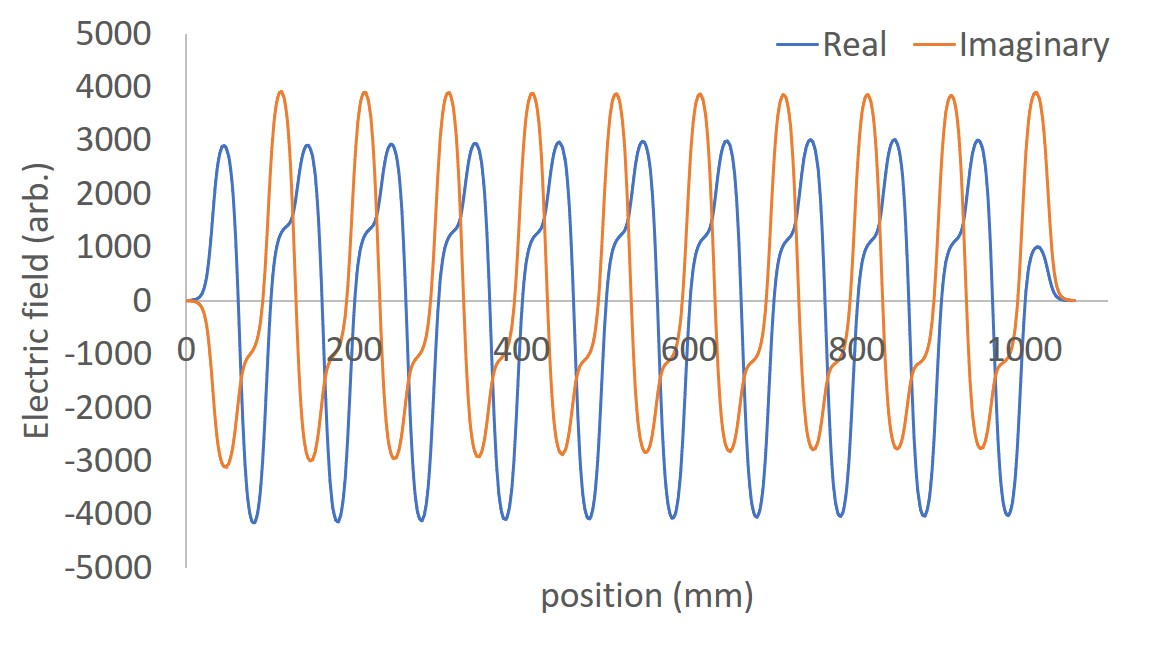
\includegraphics[width=120mm]{figures/TWS_complex.pdf}
\caption{\label{fig_TWScomplex} $2\pi/3$ 行波结构中纵向电场的实部和虚部。}
\end{figure}

\begin{figure}
\centering
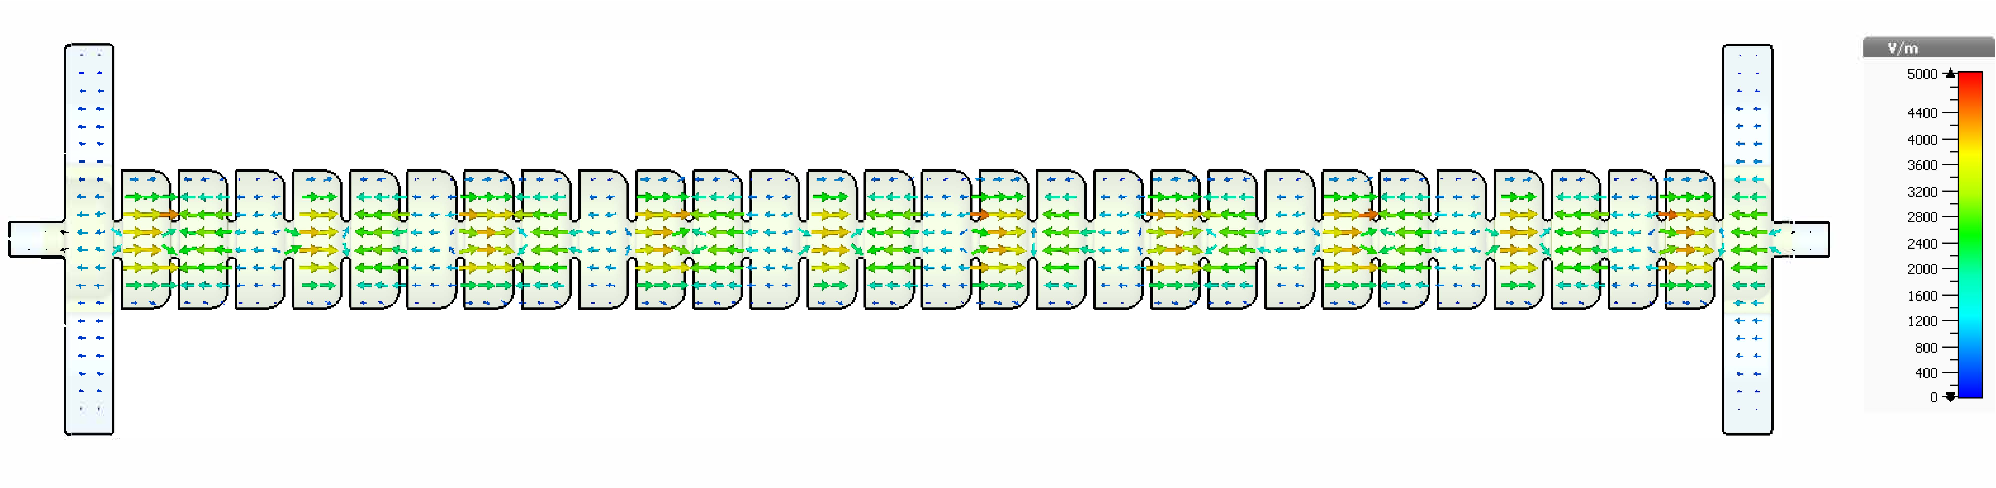
\includegraphics[width=140mm]{figures/AWAKE_TWS.pdf}
\caption{\label{fig_TWS} AWAKE 增强器的行波结构。}
\end{figure}

每个单元都有功率流入 $P_w$、由于欧姆损耗或束流加载造成的单元内功率损失，以及从该单元流出的功率。如果功率流远大于其他损耗，那么结构的带宽就更宽，腔体就会表现得像行波，且每个单元的充填时间相对于功率流经整个结构的时间而言很短。正是这种带宽的增加，使行波结构对缺陷不敏感，从而可以使用更长的结构，其长度至少可达到驻波结构的四倍。也可以对较短的结构进行加载，使群速度、进而功率流显著降低，以提高效率。在这种情况下，各单元充填得更慢，并且在充填过程中可能会出现反射，类似于行波与驻波结构之间的混合体~\cite{TERA}。
由于欧姆损耗，功率流会沿结构方向逐渐减小。群速度越低，单元中的欧姆损耗越高，因此功率流沿结构长度下降得越快。如果结构过长，则到结构末端时功率会过低，无法获得可用的梯度，因此每种结构都有一个由群速度决定的最大实际长度。如果结构过短，则结构末端的功率流会很大，并会被射频负载吸收。不过，更低的群速度也会增加每个单元的储能，因此有利于提高梯度。因此，对于给定的结构长度，应选择合适的群速度以最大化平均梯度。

如果考虑从一个单元流向下一个单元的波的匹配，那么该单元可以看作一个单独的单元，并与两个外部耦合器强耦合（分别代表与相邻单元之间的流入和流出）。在端部单元中，耦合器还必须与表观外部 Q 因子匹配，该 Q 因子代表向下一单元的功率流。与单元间功率流相关的 Q 因子 $Q_f$ 表示为
\begin{equation}
Q_f=\frac{\omega L}{v_g (1-exp(-2 \alpha L))}.
\end{equation}
由于单个单元中的衰减很小，且单元长度由相位推进决定，因此可化简为
\begin{equation}
Q_e=Q_f=\frac{c \phi_a}{v_g}.
\end{equation}
对于典型的群速度——约为光速的几个百分点——这会得到一个远低于驻波腔的 Q 值，从而带来更快的充填时间和更大的带宽。这并不是功率损耗，而是功率流，因此只要结构足够长，它仍然可以保持高效率。
\newpage
\begin{thebibliography}{99}

%\bibliography{bibliography}
%\bibliographystyle{plain}





\bibitem{Pozar}
D.M Pozar. Microwave Engineering; 3rd ed. Wiley, Hoboken, NJ, 2005.


\bibitem{Padamsee}
H. Padamsee, J Knobloch, T Hays, et al. RF Superconductivity for Accelerators, volume 2011. Wiley
Online Library, 2008.



\bibitem{wangler}
T. P. Wangler. RF Linear Accelerators, Second Edition. Wiley, 2008

\bibitem{DLATHz}
MT Hibberd, AL Healy, DS Lake, V Georgiadis, EJH Smith, OJ Finlay, TH Pacey, JK Jones,
Y Saveliev, DA Walsh, et al. Terahertz-driven acceleration of a relativistic 35 MeV electron beam.
In 2019 44th International Conference on Infrared, Millimeter, and Terahertz Waves (IRMMW-THz),
pages 1–2. IEEE, 2019.

\bibitem{TWS}
C. Nantista, S. Tantawi, and V. Dolgashev. Low-field accelerator structure couplers and design
techniques. Physical Review Special Topics: Accelerators and Beams, 7(7):072001, 2004.
12

\bibitem{Kroll}
N. M. Kroll, C. K. Ng, and D. C. Vier. Applications of time domain simulation to coupler design for
periodic structures. In Proceedings of 20th International Linac Conference, Linac 2000, Monterey,
USA, pages 614–617.


\bibitem{AWAKEboost}
K Pepitone, S Doebert, G Burt, E Chevallay, N Chritin, C Delory, V Fedosseev, Ch Hessler, G Mc-
Monagle, Oznur Mete, et al. The electron accelerator for the AWAKE experiment at CERN. Nuclear
Instruments and Methods in Physics Research Section A: Accelerators, Spectrometers, Detectors and
Associated Equipment, 829:73–75, 2016.


\bibitem{TERA}
S Benedetti, A Grudiev, and A Latina. High gradient linac for proton therapy. Physical Review
Accelerators and Beams, 20(4):040101, 2017.

%\bibitem{bib:Wolski} 


\end{thebibliography}

\end{document}